\newpage

\section{Les arbres binomiaux}

L'approche par arbres binomiaux, souvent associée au modèle de Cox-Ross-Rubinstein, propose une méthode discrète et intuitive pour modéliser la dynamique du cours d'une action et évaluer les options.

Contrairement aux modèles continus qui peuvent sembler abstraits, ce modèle repose sur une idée simple : le temps est découpé en périodes, et à chaque étape, le prix ne peut aller que dans deux directions. C'est cette simplicité qui permet de comprendre la mécanique profonde de l'évaluation d'options. Notons d'ailleurs que lorsque la durée des périodes tend vers 0, ce modèle converge mathématiquement vers la loi log-normale utilisée dans le modèle de Black \& Scholes.

\subsection{Modélisation à une période}

Commençons par le cas le plus élémentaire : une seule période de temps $T$.
Soit une action de prix actuel $S_0$ et une option sur cette action (par exemple un Call) de valeur inconnue $f$.

L'hypothèse fondamentale est que le cours suit une marche aléatoire multiplicative. À l'issue de la période $T$, deux états de la nature sont possibles :
\begin{itemize}
    \item \textbf{État Haut (Up) :} Le prix monte à $S_u = S_0 \cdot u$ (avec $u > 1$).
    \item \textbf{État Bas (Down) :} Le prix descend à $S_d = S_0 \cdot d$ (avec $d < 1$).
\end{itemize}

Les payoffs (flux) de l'option à l'échéance dépendront de ces états : $f_u$ si le marché monte, et $f_d$ s'il baisse.

\begin{center}
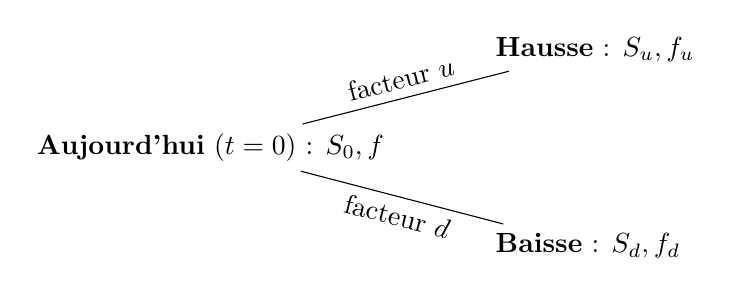
\begin{tikzpicture}[grow=right, sloped, level distance=3.5cm, sibling distance=2.5cm]
    \node[left] {\textbf{Aujourd'hui} ($t=0$) : $S_0, f$}
    child {
        node[right] {\textbf{Baisse} : $S_d, f_d$}
        edge from parent
        node[below] {facteur $d$}
    }
    child {
        node[right] {\textbf{Hausse} : $S_u, f_u$}
        edge from parent
        node[above] {facteur $u$}
    };
\end{tikzpicture}
\end{center}

\subsection{Le mécanisme de couverture (Delta-Hedging)}

Comment déterminer la valeur $f$ de l'option aujourd'hui ? L'intuition géniale de ce modèle ne repose pas sur la spéculation de la direction du marché, mais sur la **réplication**.

Nous allons construire un portefeuille fictif $\Pi$ composé de :
\begin{itemize}
    \item Une position longue sur $\Delta$ actions.
    \item Une position courte sur 1 option (vente de l'option).
\end{itemize}

La valeur de ce portefeuille à l'instant $T$ est aléatoire :
$$ \Pi_T = \begin{cases} S_0 u \Delta - f_u & \text{si le marché monte} \\ S_0 d \Delta - f_d & \text{si le marché baisse} \end{cases} $$

L'objectif est de choisir $\Delta$ de manière à **éliminer le risque**. Nous voulons que la valeur du portefeuille soit identique, que le marché monte ou qu'il descende.

\begin{proofbox}[Calcul du Ratio de Couverture $\Delta$]
Pour rendre le portefeuille sans risque, nous égalisons les deux issues possibles :
$$ S_0 u \Delta - f_u = S_0 d \Delta - f_d $$

En regroupant les termes en $\Delta$, nous obtenons :
$$ \Delta (S_0 u - S_0 d) = f_u - f_d $$

Ce qui nous donne la formule du Delta :
$$ \Delta = \frac{f_u - f_d}{S_u - S_d} $$
\end{proofbox}

\textbf{Interprétation économique :} Le ratio $\Delta$ représente la sensibilité du prix de l'option aux variations du sous-jacent. En détenant $\Delta$ actions pour chaque option vendue, les gains sur l'action compensent exactement les pertes sur l'option (et inversement).

\subsection{Dérivation de la formule de valorisation}

Puisque nous avons construit un portefeuille sans risque, il ne doit pas exister d'opportunité d'arbitrage. Par conséquent, ce portefeuille doit rapporter exactement le taux sans risque $r$. Si ce n'était pas le cas, des investisseurs pourraient réaliser un profit infini sans risque.

La valeur actuelle du portefeuille ($\Pi_0$) doit donc être égale à sa valeur future certaine actualisée au taux $r$ :
$$ \underbrace{S_0 \Delta - f}_{\text{Coût initial}} = \underbrace{(S_0 u \Delta - f_u)}_{\text{Valeur future certaine}} \cdot e^{-rT} $$

C'est ici que nous intégrons le calcul complet pour isoler le prix de l'option $f$.

\begin{proofbox}[Détail du calcul algébrique]
Notre but est d'exprimer $f$ en fonction des paramètres connus. Partons de l'équation d'absence d'arbitrage ci-dessus :

\textbf{Étape 1 : Isoler $f$}
$$ f = S_0 \Delta - (S_0 u \Delta - f_u) e^{-rT} $$
Factorisons les termes contenant $\Delta$ :
$$ f = S_0 \Delta (1 - u e^{-rT}) + f_u e^{-rT} $$

\textbf{Étape 2 : Substitution du Delta}
Remplaçons $\Delta$ par sa valeur calculée précédemment $\frac{f_u - f_d}{S_0(u - d)}$ :
$$ f = S_0 \left[ \frac{f_u - f_d}{S_0(u - d)} \right] (1 - u e^{-rT}) + f_u e^{-rT} $$
Les termes $S_0$ s'annulent. Pour simplifier, factorisons l'ensemble par le facteur d'actualisation $e^{-rT}$. Notez que le terme $(1 - u e^{-rT})$ devient $(e^{rT} - u)$ une fois $e^{-rT}$ sorti en facteur :
$$ f = e^{-rT} \left[ \frac{f_u - f_d}{u - d} (e^{rT} - u) + f_u \right] $$

\textbf{Étape 3 : Réarrangement en probabilités}
Développons pour regrouper les termes multipliant $f_u$ et ceux multipliant $f_d$ :
$$ f = e^{-rT} \left[ f_u \left( \frac{e^{rT} - u}{u - d} + 1 \right) + f_d \left( \frac{-(e^{rT} - u)}{u - d} \right) \right] $$

Simplifions le coefficient devant $f_u$ (mise au même dénominateur) :
$$ \frac{e^{rT} - u + u - d}{u - d} = \frac{e^{rT} - d}{u - d} $$

Nous définissons cette quantité comme étant $p$. On constate alors que le coefficient devant $f_d$ est exactement $1-p$.
\end{proofbox}

\subsection{La probabilité risque-neutre}

Le calcul précédent nous permet d'aboutir à une formule d'une élégance remarquable, qui ressemble à une espérance mathématique.

\begin{theorembox}[Formule de valorisation binomiale]
La valeur de l'option est l'espérance actualisée de ses flux futurs sous la probabilité risque-neutre $p$ :
$$ f = e^{-rT} [p f_u + (1 - p) f_d] $$
Où la probabilité $p$ est définie par :
$$ p = \frac{e^{rT} - d}{u - d} $$
\end{theorembox}